\section{Results}
The model receives a reward ($+1$) every second that trunk lean is less than $30^{\circ}$. Figure \ref{fig:boxplot} shows variation of reward with respect to number of training iterations for $10$, $20$, $30$ and $40$ million. In this figure, red line indicates mean value, horizontal lines maximum and minimum values. Likewise, the reward that model gets with $20$ million is greater than with $10$ million. This is because the model learns to walk better with more training time. However, the reward that model gets with $30$ and $40$ million is less than with $20$ million. This is because model is trying/learning to use both legs instead of just one\footnote{visual material of the training of the two-legged robot in \url{https://www.youtube.com/watch?v=Vt20_SWR2xI&ab_channel=LucaBorgonovi}}.


\begin{figure}
	\centering
	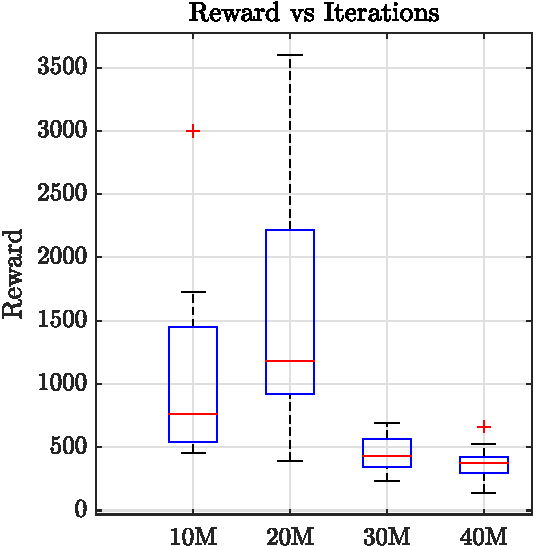
\includegraphics{images/reward_vs_iter.pdf}
	\caption{Performance of trained model to keep the trunk lean below $30^{\circ}$.}
	\label{fig:boxplot}
\end{figure}

